\subsection{Pengujian \emph{depth camera}}
\label{subsec:depthcameratesting}

\begin{figure} [ht]
  \centering
  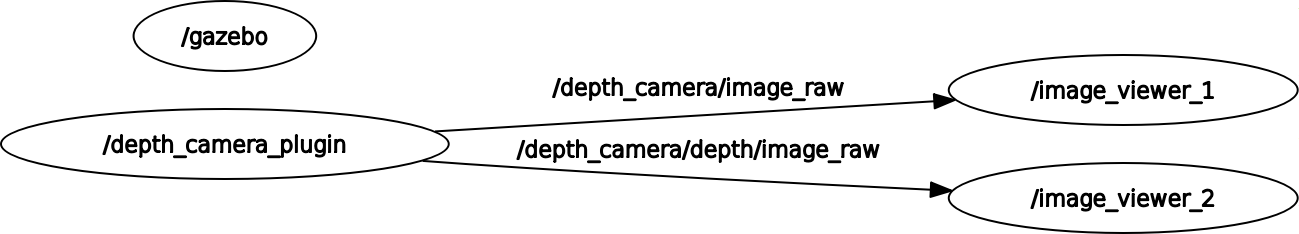
\includegraphics[width=0.45\textwidth]{figures/rosgraph/depth-camera-sim.png}
  \IfLanguageName{english}{
    \caption{Node scheme of the depth camera testing in the simulation.}
  }{
    \caption{Skema \emph{node} dari pengujian \emph{depth camera} di simulasi.}
  }
  \label{fig:rosgraphdepthcamerareal}
\end{figure}

\begin{figure} [ht]
  \centering
  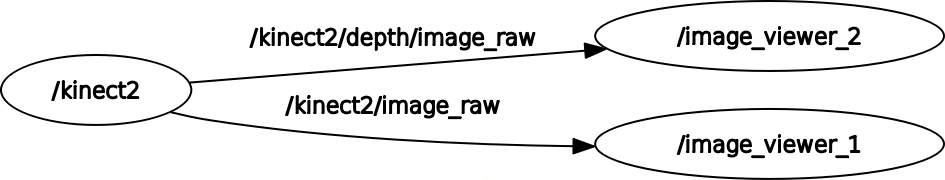
\includegraphics[width=0.45\textwidth]{figures/rosgraph/depth-camera-real.png}
  \IfLanguageName{english}{
    \caption{Node scheme of the depth camera testing on the real robot.}
  }{
    \caption{Skema \emph{node} dari pengujian \emph{depth camera} pada robot fisik.}
  }
  \label{fig:rosgraphdepthcamerareal}
\end{figure}


Pengujian \emph{depth camera} dilakukan untuk menguji kemampuan \emph{depth camera} di simulasi dalam mensimulasikan perangkat \emph{depth camera},
  sekaligus menguji abstraksi perangkat yang ada pada ROS 2.
Pengujian ini dilakukan dengan menjalankan dua buah \emph{node} \lstinline{image_viewer} yang masing-masing akan menerima data citra warna dan citra kedalaman.
Seperti yang terlihat pada gambar \ref{fig:rosgraphdepthcamerasim},
  di simulasi,
  masing-masing \emph{node} \lstinline{image_viewer} akan menerima data citra warna melalui \emph{topic} \lstinline{/depth_camera/image_raw} dan data citra kedalaman melalui \emph{topic} \lstinline{/depth_camera/depth/image_raw}.
Sedangkan untuk pengujian di dunia nyata,
  seperti yang terlihat pada gambar \ref{fig:rosgraphdepthcamerareal},
  peran dari \emph{node} \lstinline{depth_camera_plugin} akan digantikan oleh \emph{node} \lstinline{v4l2_camera} yang akan mengirimkan data yang berasal dari perangkat Kinect V2 yang ada pada robot fisik.

\begin{figure} [ht]
  \centering
  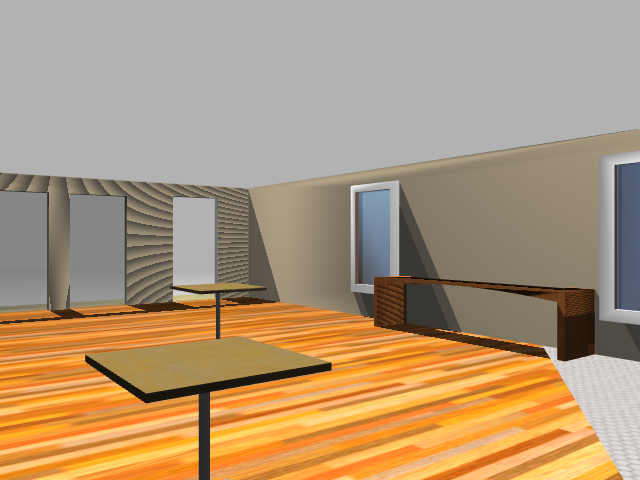
\includegraphics[width=0.225\textwidth]{figures/depth-camera/sim-rgb.png}
  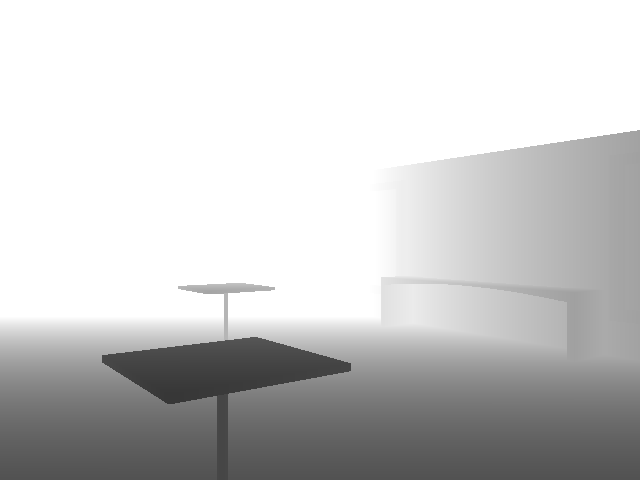
\includegraphics[width=0.225\textwidth]{figures/depth-camera/sim-depth.png}
  \IfLanguageName{english}{
    \caption{Comparison of the depth camera capture results in the simulation.}
  }{
    \caption{Perbandingan hasil tangkapan \emph{depth camera} di simulasi.}
  }
  \label{fig:depthcameraresultsim}
\end{figure}


Hasilnya,
  seperti yang terlihat pada gambar \ref{fig:depthcameraresultsim},
  \emph{node} \lstinline{image_viewer} menampilkan data yang diterima dari simulasi dimana gambar kiri (\ref{fig:depthcameraresultsimrgb}) menunjukkan citra dengan tampilan berwarna,
  sedangkan gambar kanan (\ref{fig:depthcameraresultsimdepth}) menunjukkan citra kedalaman dengan tampilan hitam putih.
Pada citra kedalaman,
  terangnya suatu titik pada citra tersebut menunjukkan posisi yang semakin jauh dari jangkauan titik pusat kamera.
Sebagai contoh,
  gelapnya bentuk meja pada citra tersebut menunjukkan posisi objek tersebut lebih dekat dibandingkan objek yang lain.

\begin{figure} [ht]
  \centering
  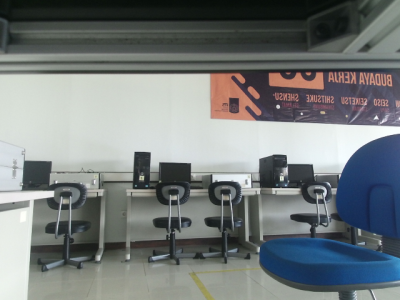
\includegraphics[width=0.225\textwidth]{figures/depth-camera/real-rgb.png}
  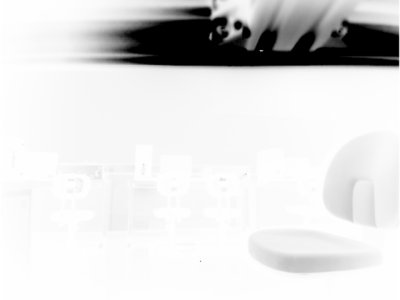
\includegraphics[width=0.225\textwidth]{figures/depth-camera/real-depth.png}
  \IfLanguageName{english}{
    \caption{Comparison of the depth camera capture results on the real robot.}
  }{
    \caption{Perbandingan hasil tangkapan \emph{depth camera} pada robot fisik.}
  }
  \label{fig:rosgraphdepthcamerareal}
\end{figure}


Sedangkan,
  pada robot fisik hasil yang didapatkan juga relatif sama.
Seperti yang terlihat pada gambar \ref{fig:depthcameraresultreal},
  gambar kiri (\ref{fig:depthcameraresultrealrgb}) menunjukkan citra warna sedangkan gambar kanan (\ref{fig:depthcameraresultrealdepth}) menunjukkan citra kedalaman.
Namun,
  pada gambar tersebut,
  citra kedalaman memiliki hasil yang lebih terang,
  hal ini terjadi karena jangkauan perangkat Kinect V2 yang lebih dekat (4.5 meter) dibandingkan jangkauan yang diatur pada \emph{depth camera} yang ada di simulasi.
